\section{Introduction}

\begin{frame}{\insertsection}{}
	\begin{itemize}
		\item 
	\end{itemize}
\end{frame}

\begin{frame}{\insertsection}{What is topic modeling?}
	\begin{itemize}
		\item Imagine going through $139,060$ articles, manually
		\item With the goal of finding all sports article.
	\end{itemize}
\end{frame}

\begin{frame}{\insertsection}{What is topic modeling?}
	\begin{itemize}
		\item Topic modeling
  		\begin{itemize}
			\item Data has arisen from a generative process
			\item Discover main themes within a collection of documents.
		\end{itemize}
	\end{itemize}
\end{frame}

\begin{frame}{\insertsection}{What is topic modeling?}
	\begin{figure}
		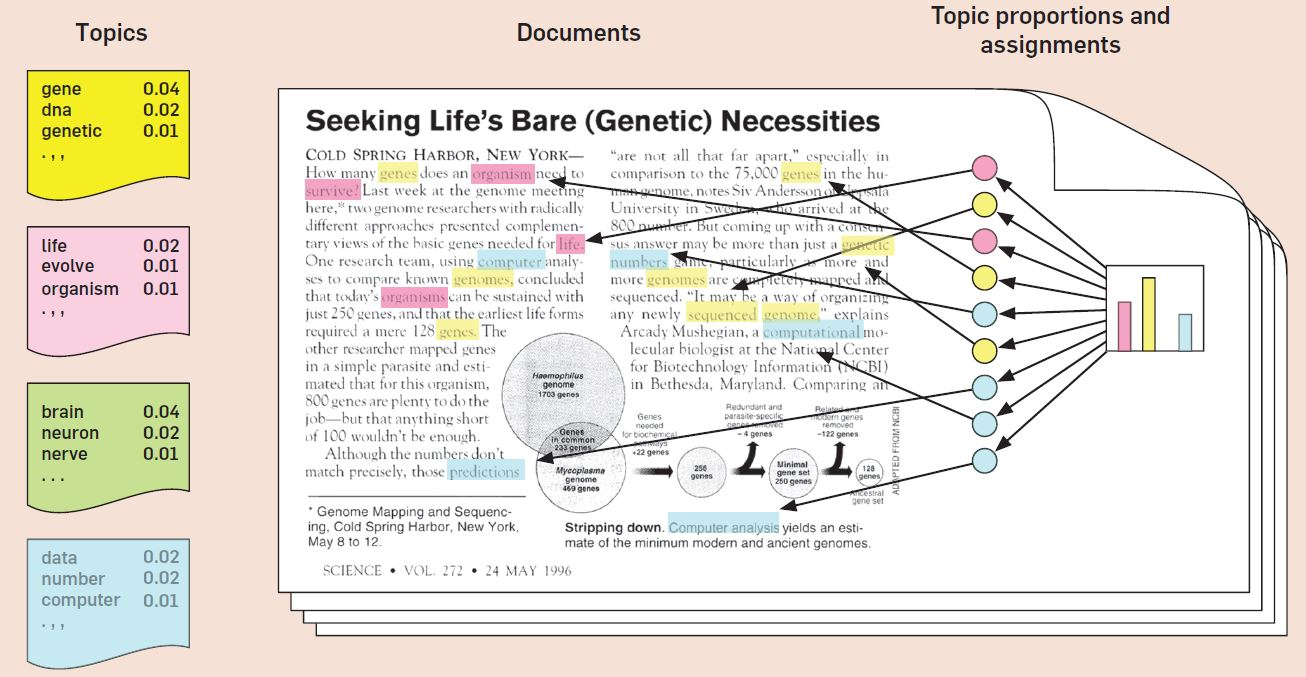
\includegraphics[width=\textwidth]{figures/topic_modeling_visual.JPG}
		\let\thefootnote\relax\footnote{\tiny{http://www.cs.columbia.edu/~blei/papers/Blei2012.pdf}}
	\end{figure}
\end{frame}

\begin{frame}{\insertsection}{Topic modeling using news articles}
	\begin{figure}
		
\includegraphics[width=\textwidth]{figures/danish_newspapers.jpg}
		\let\thefootnote\relax\footnote{\tiny{https://www.fyidenmark.com/denmark-newspapers.html}}
	\end{figure}
\end{frame}

\section{Dataset}

\begin{frame}{\insertsection}{Nordjyske}
	\begin{figure}
		
\includegraphics[width=0.6\textwidth]{figures/nordjyske-medier.png}
		\let\thefootnote\relax\footnote{\tiny{https://addfocus.dk/nordjyske-medier-2/}}
	\end{figure}
	\begin{itemize}
		\item 2017-2019
		\item News articles
		\item Multiple \textbf<2>{metadata} fields
	\end{itemize}
\end{frame}


\begin{frame}{\insertsection}{The three chosen metadata}
	\begin{itemize}
		\item Author
		\item Category
		\item Taxonomy
	\end{itemize}
\end{frame}

\subsection{Author}

\begin{frame}{\insertsubsection}{Metadata description}
	\begin{itemize}
		\item The person who has written the article
		\item $184$ unique authors (after preprocessing)
	\end{itemize}
	\vspace{2em}
	\only<2>{
		\begin{itemize}
			\item What impact does the author have on the underlying topics?
		\end{itemize}
	}
\end{frame}
